\documentclass{rapport}
\usepackage{lipsum}
\usepackage{tikz}
\usepackage{wrapfig}
\usepackage{caption}
\title{Rapport UCL - Template} %Titre du fichier

\begin{document}

%----------- Informations du rapport ---------

\unif{EURECOM}
\titre{S5 PROJECT REPORT :\\ 
\begin{center}

\includegraphics[width=0.3\linewidth]{logo_visuwalk.png} 
\end{center}VISUWALK} %Titre du fichier .pdf
% \cours{Nom du cours} %Nom du cours
% \sujet{Sujet du rapport} %Nom du sujet


%----------- Initialisation -------------------
        
\fairemarges %Afficher les marges
\fairepagedegarde %Créer la page de garde
\tableofcontents%Créer la table de matières
\newpage

%------------ Corps du rapport ----------------
\section{Abstract}

For this semester project, to aid the 2.2 billion visually impaired persons in the world, we were asked to develop a system capable of guiding the latter following a line.\\
The tools we were given are a Raspberry Pi and its camera. The main goals of this project are the following :\\
detect the line from the Raspberry Pi’s camera\\
process the information given by the line\\
generate sound cues to guide the user\\

\section {User manual}

\section{Technical manual}

\subsection{Introduction to the Raspberry Pi and Matlab/Simulink
}
    
The first steps towards this project were to connect the Raspberry Pi to our computers and to discover Matlab, which were not easy tasks.
The whole installation was quite lengthy, and did not work for most of us. And if it did work, we then had to connect the camera to the Raspberry Pi, which was also quite hard. So hard that we even thought our camera was broken, until we tested it on other computers, which took a lot of time. In the end, we were left with only 2 Raspberry Pi connected and 2 cameras (Alexandre bought one himself).
Concerning Matlab and Simulink, some of us had already used these softwares, but only on surface-level, so we pretty much had to learn from scratch how to use them and more specifically, how to use them with the Raspberry Pi. And this last part was complicated, leading us to this next paragraph.

\subsection{Choosing between Python and Matlab/Simulink
}

The option of using Python showed up because other groups had issues just like us and switched to Python. Thus, we talked about the switch, and decided not to switch completely as we had already advanced on the Matlab code. Instead, we let Guillaume,in parallel, try to do the video processing part (that was done on Matlab) on Python, to see how easier it would be.
It was much easier and produced better results.And so we were left with one last question : should we also do the sound generation part on Python ?
We were quite reluctant at first, given that almost the whole code was already done in Simulink and that switching and translating it all would take an important amount of time. Besides, we searched and found multiple ways to make a bridge between Python and Simulink. But time was ticking and we still had not found a way to make any of these bridges work correctly, so we made the switch. And it did not take as long as we expected, despite the issues we encountered. 
Still, we found some interesting features like the C code generation, which would be used to embed the program on a portable system. Knowing that shared memory in C is possible and probably easier than in Matlab, we searched for a way to use shared memory in Python, and to manually modify the C generated code to implement the share of memory between the sound generation part and the Python video processing, so that the second could indicate the direction to the first.

\subsection{Image processing part}

The first step toward computing the image and giving an angle is the image acquisition. We use the python library \verb|picamera| in order to get the camera's images, at a quite low quality, because it has proven to be more time-efficient.

% Gui tu peux changer le wrapfigure par des colonnes ou tout ce que tu veux
\begin{center}
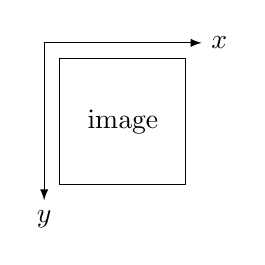
\begin{tikzpicture}[scale=2]
\draw[-latex] (0,0) -- (1,0);
\draw[-latex] (0,0) -- (0,-1);
\draw (0.1,-0.1) rectangle (0.9, -0.9);
\draw (0.5,-0.5) node {image};
\draw (1,0) node[right] {\(x\)};
\draw (0,-1) node[below] {\(y\)};
\end{tikzpicture}
\captionof{figure}{OpenCV x and y axis representation}
\end{center}


The frames are then read by openCV and converted into grey. OpenCV represents images with matrices whose indexes may also be seen as coordinate of the following base. An image pixel is then characterized by its coordinate in the following order: \verb|image[y,x]| (matrix line, matrix column).

We then apply a bilateral filter to the image, as it is a filter that preserve the sharp edges and smooth the rest of the image: this is exactly what we need, especially as there is a pattern with lines on the carpet of the Marconi amphiteater that needs to be removed.

% inserer capture de l'image filtree ?

After having a clear image of the line, we apply the Hough transform which will give us a set of straight lines detected on the image. But before calculating any angle, we need to reorient the lines accordingly to our purpose. Indeed, openCV will return us vectors that are oriented towards increasing \(x\), but we need to have them all in the same directon as \(y\), because the user moves on the y axis.

% place le ou tu veux comme tu veux Gui
\begin{center}
    \begin{tikzpicture}[scale=2]
  \draw[-latex] (0,0) -- (0,-1);
  \draw (0,-1) node[below] {\(y\)};

  \draw (0.7,-0.3) -- (1.2,-1.1);
  \draw (1.2,-1.5) -- (0.7,-2.3);

  \draw[->] (1.4, -0.6) -- (1.6, -0.6);
  \draw[->] (1.4, -1.9) -- (1.6, -1.9);

  \draw[->] (2,-0.3) -- (2.5,-1.1);
  \draw[<-] (2.5,-1.5) -- (2,-2.3);

  \draw[->] (2.7, -1.9) -- (2.9, -1.9);

  \draw[->] (3.7,-1.5) -- (3.2,-2.3);
\end{tikzpicture}
\captionof{figure}{popo}
\end{center}

\subsection{Description of source files directory}

In the folder of the source code archive, you will find the \verb|rasp_prod| folder, containing the production source code for the raspberry device, the \verb|improc| and \verb|soundproc| folder containing our test codes for development, and the case folder containing some aborted concept protection and fixation covers for the raspberry. (...)



\end{document}
